\subsubsection{Smartphone als Master}
	Ein Smartphone vereint mehrere für die Realisation des Produkts benötigte Komponenten (Kamera, drahtlose Schnittstelle, Recheneinheit, Endsignalausgabe) 
	in einem Gerät. Des Weiteren sind heutige Smartphones verhältnismässig leistungsfähig, die Berechnungen für die Objekterkennung 
	können direkt auf dem Gerät erfolgen und durch den USB-Port wird eine sichere Verbindung zum Controller gewährleistet. Die Alternative, einzelne Module (Kamera, drahtlose Schnittstelle, Recheneinheit) zu verbauen, 
	gewährleistet eine erhöhte Flexibilität, allerdings verbunden mit steigendem Aufwand und höherem Preis. 
	Zudem hätte die Verwendung von Einzelmodulen unter Umständen eine Gewichtszunahme zur Folge, da keine vergleichbare Kompaktheit wie bei einem Smartphone besteht. 
	Der Einsatz eines Smartphones bietet im Vergleich zu einzelnen Modulen somit entscheidende Vorteile.\\
	\\
	Es ist wichtig, dass die Kamera das Spielfeld komplett erfassen kann, weswegen das Smartphone vorne am Gerät angebracht wird. 
	Eine Befestigung an der Front des Gerätes bietet sich an, da dort eine hohe Stabilität vorhanden ist, 
	was für eine optimale Bildaufnahme wichtig ist.\\
	\\
	Falls die Korberkennung aus irgendeinem Grund nicht auf dem Smartphone implementiert werden kann, 
	wird die Berechnung auf einem externen PC durchgeführt. Eine Kamera würde als Webcam am PC 
	angeschlossen. Die Montage würde am selben Ort wie das Smartphone vorgenommen. Die Kommunikation 
	zwischen PC und dem Controller würde wie beim Smartphone über USB realisiert.
	%
	\paragraph{Korberkennung}$~~$\vspace{2mm}\\
		Für die Bestimmung der Position des Korbes wurde ein Algorithmus entwickelt und in Java implementiert. Dieser ist in Abbildung \ref{fig:KorberkennungFlowchart} grafisch dargestellt.
		Der Algorithmus bedient sich des Umstandes, dass der Korb deutlich dunkler als der Hintergrund ist. 
		Um mit dem von der Kamera zuvor aufgenommenen Bild arbeiten zu können, müssen die Ränder abgeschnitten werden 
		(vor allem links und rechts geht der Bildbereich über das Spielfeld hinaus, was das Resultat verfälschen könnte). 
		Als zweiter Schritt wird über sämtliche Pixel des Bildes iteriert. Dabei wird für jedes Pixel die Helligkeit bestimmt 
		anhand einer vordefinierten Schwelle entschieden, ob es zum Hintergrund (heller) oder zum Korb (dunkel) gehört. 
		Anschliessend wird der Schwerpunkt der dunklen Pixel bestimmt und anhand des gefundenen Schwerpunktes entweder
		von links oder von rechts her in einem bestimmten horizontalen Bereich (der Korb befindet sich immer auf der selben Höhe)
		über die Pixel iteriert um dabei eine feste Kontur zu finden. Diese feste Kontur wird dabei definiert durch eine
		bestimmte Anzahl weisse Pixel, auf welche wiederum eine Menge schwarzer Pixel folgen muss. 
		Da dieser Prozess immer in derselben horizontalen Ebene stattfindet kann durch eine abschliessende Berechnung 
		der Mittelpunkt des Korbes und der damit verbundene Winkel des Ballwerfers zum Korb trigonometrisch bestimmt werden.
		\begin{figure}[h!]
			\centering
			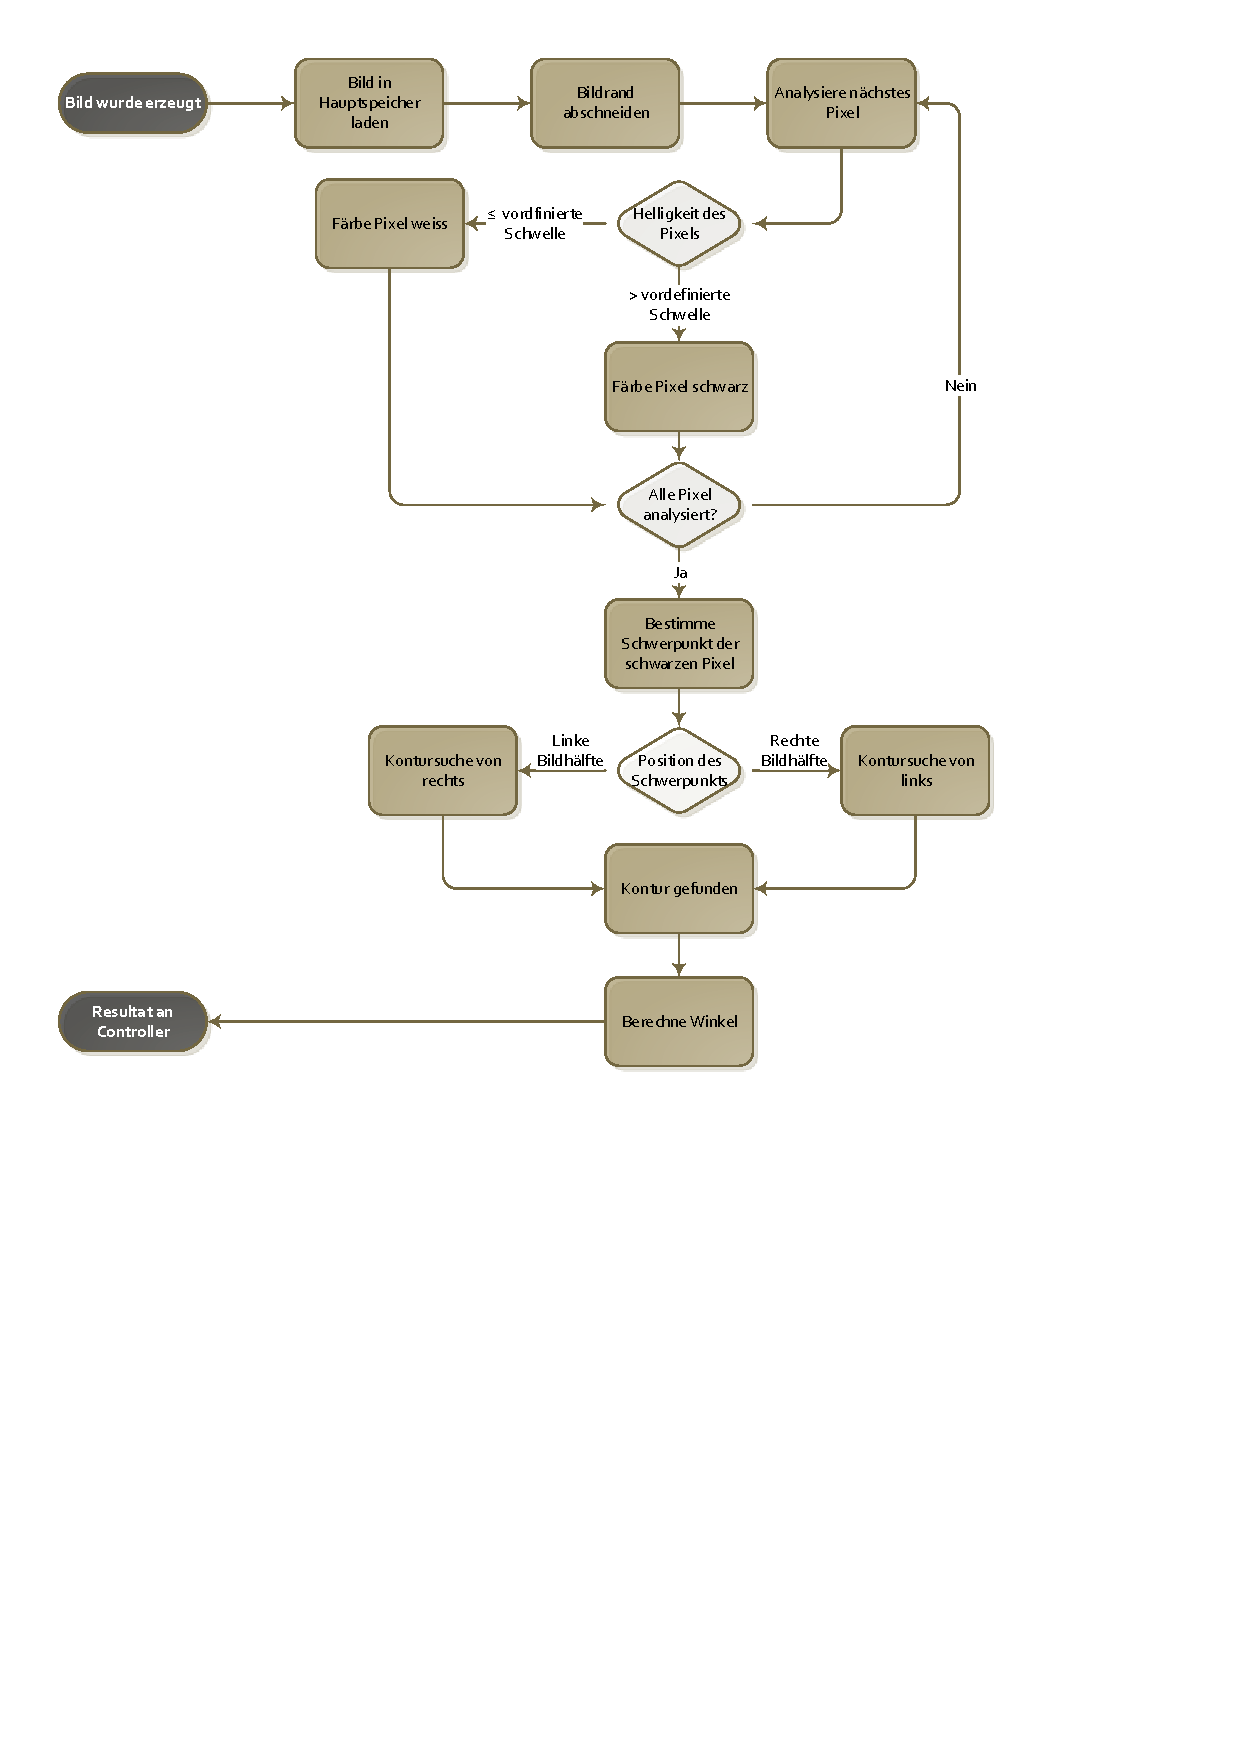
\includegraphics[width=1\textwidth,clip,trim=9mm 115mm 41mm 9mm]
			{Enddokumentation/Loesungskonzept/Bilder/Flowchart_Korberkennung.pdf}
			\caption{Ablaufdiagramm zum Korberkennungs-Algorithmus}
			\label{fig:KorberkennungFlowchart}
		\end{figure}